\documentclass[]{auvsi_doc}
\setkeys{auvsi_doc.cls}{
	AUVSITitle={Design Summary},
%	AUVSIRevision=0.0,
%	AUVSIDescription={Created},
%	AUVSIAuthor={Kameron Eves},
%	AUVSIChecker={[Checker]},
	AUVSILogoPath={./figs/logo.pdf},
%	AUVSIDocID={AF-004}
}

% include extra packages, if needed
\usepackage{makecell}
\usepackage{multirow}

% Remove Heading Numbers
\setcounter{secnumdepth}{0}

\begin{document}
\begin{AUVSITitlePage}
\begin{artifacttable}
	\entry{TW-002, 0.1, 12-03-2018, Created, Kameron Eves, Andrew Torgesen}
	\entry{TW-002, 0.2, 12-10-2018, Added payload delivery sections, Andrew Torgesen, [CHECKER]}
\end{artifacttable}
\end{AUVSITitlePage}


\section{ Introduction}

Each year, the Association for Unmanned Vehicle Systems International (AUVSI) hosts a Student Unmanned Aerial Systems (SUAS) competition. This year’s competition will be held June 12th to 15th, 2019 and BYU will be sending a team to compete.

The aircraft entered into the competition are judged primarily on a demonstration of ability to autonomously complete a mission which includes the following tasks:

\begin{itemize}
	\item\textbf{Fly Waypoint Path} - Fly waypoints given to the the team just prior to the competition. In this process, and throughout the entire mission, the aircraft must avoid virtual obstacles and stay within boundaries (both horizontal and vertical).
	\item\textbf{Visual Target Classification} - Capture an image of several targets within a search area and report to the judges the shape, color, alpha-numeric character, alpha-numeric character color, and geolocation of each target.
	\item\textbf{Payload Delivery} - Drop on a specified location, an unmanned ground vehicle (UGV) that itself carries a small water bottle. Then, carrying its the water bottle, the UGV must drive to a second specified location.
\end{itemize}

In order, to accomplish these tasks our team has decided upon the following objective statement:

\begin{quote}
Improve upon last year’s BYU AUVSI unmanned aerial system (UAS) by improving path planning, obstacle avoidance, visual object detection, and payload delivery by April 1, 2019 with a budget of \$3,500 and 2,500 man hours.
\end{quote}

We have stipulated several key success measures which are enumerated in Table~\ref{tab:key_measures}. Additional market requirements, performance measures, ideal values, and target values are included in RM-001.

\begin{table}[H]
	\centering
	\caption{Key success measures for the UAS}\label{tab:key_measures}
\begin{tabular}{|P{7.1cm}|>{\centering\arraybackslash}P{0.75cm}|>{\centering\arraybackslash}P{0.75cm}>{\centering\arraybackslash}P{0.75cm}>{\centering\arraybackslash}P{0.75cm}|>{\centering\arraybackslash}P{0.75cm}>{\centering\arraybackslash}P{0.75cm}>{\centering\arraybackslash}P{0.75cm}|}
	\multicolumn{8}{c}{\textbf{\underline{Key}}} \\
		\multicolumn{8}{l}{\textbf{Performance:} \textbf{SG} = Stretch Goal, \textbf{A} = Excellent,	\textbf{B} = Good,	\textbf{C} = Fair}  \\
		\multicolumn{8}{l}{\textbf{Acceptable:} \textbf{L} = Lower, \textbf{I} = Ideal,	\textbf{U} = Upper}\\
	\hline
	\rowcolor[HTML]{C0C0C0}
	 & \multicolumn{4}{c|}{\textbf{Performance}} &\multicolumn{3}{c|}{\textbf{Acceptable}}  \\\rowcolor[HTML]{C0C0C0}
	\multirow{-2}{*}{ \textbf{Measures (units)}} &{\textbf{SG}} & {\textbf{A}} & {\textbf{B}} & {\textbf{C}} & {\textbf{L}} & {\textbf{I}} & {\textbf{U}} \\

	\hline
	\textbf{Obstacles Hit (\#)} & 0 & 1 & 3 & 5 & 0 & 0 & 5 \\
	\hline
	\textbf{Average Waypoint Proximity (ft)} & 5 & 20 & 25 & 30 & 0 & 0 & 100 \\
	\hline
	\textbf{Characteristics Identified (\%)} & 80 & 40 & 30 & 20 & 20 & 100 & 100 \\
	\hline
	\textbf{Airdrop Accuracy (ft)} & 5 & 25 & 50 & 75 & 0 & 0 & 75 \\
	\hline
	\textbf{Number of Manual Takeovers (\#)} & 0 & 1 & 2 & 3 & 0 & 0 & 3 \\
	\hline
\end{tabular}
\end{table}


\section{Description of Design}
\subsection{Airframe}
The My Fly Dream Nimbus Pro airframe was selected as this year's airframe. With a wingspan of 1.95~m and fuselage capacity of 8,000~cc, it is significantly larger than last year's airframe. The total airframe weight with components and a 1~kg UGV is 5.365~kg. It should sport aerodynamic characteristics similar to last year's plane, with improved stall speed. Electrical components like the flight controller board, RC antenna, and GPS have been spread out in the spacious fuselage to minimize signal interference and noise caused by coils of wire and antennae, while maintaining an optimal CG placement. See Fig. \ref{airframe} for a photo of the airframe, and Fig. \ref{components} for a photo of component placement.
%The larger fuselage capacity has a 12~cm x 12~cm x `23~cm space for the UGV: a huge improvement over last year's design, in which the water bottle was attached to the outside for lack of space inside the airframe.
\begin{figure}[h!]
	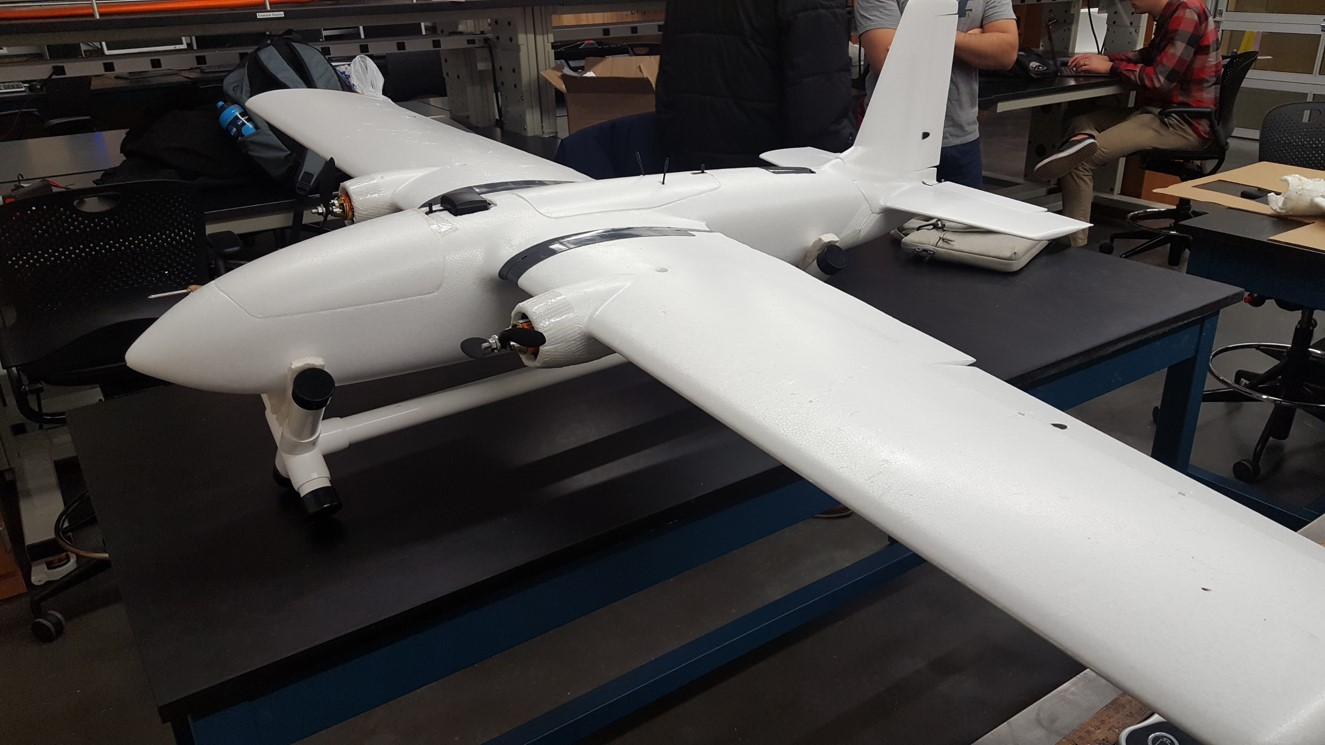
\includegraphics[scale=0.6]{figs/airframe.jpg}
	\centering
	\caption{The new airframe boasts a large wingspan, large fuselage, and easily removable wings and tail.}
	\label{airframe}
\end{figure}
\begin{figure}[h!]
	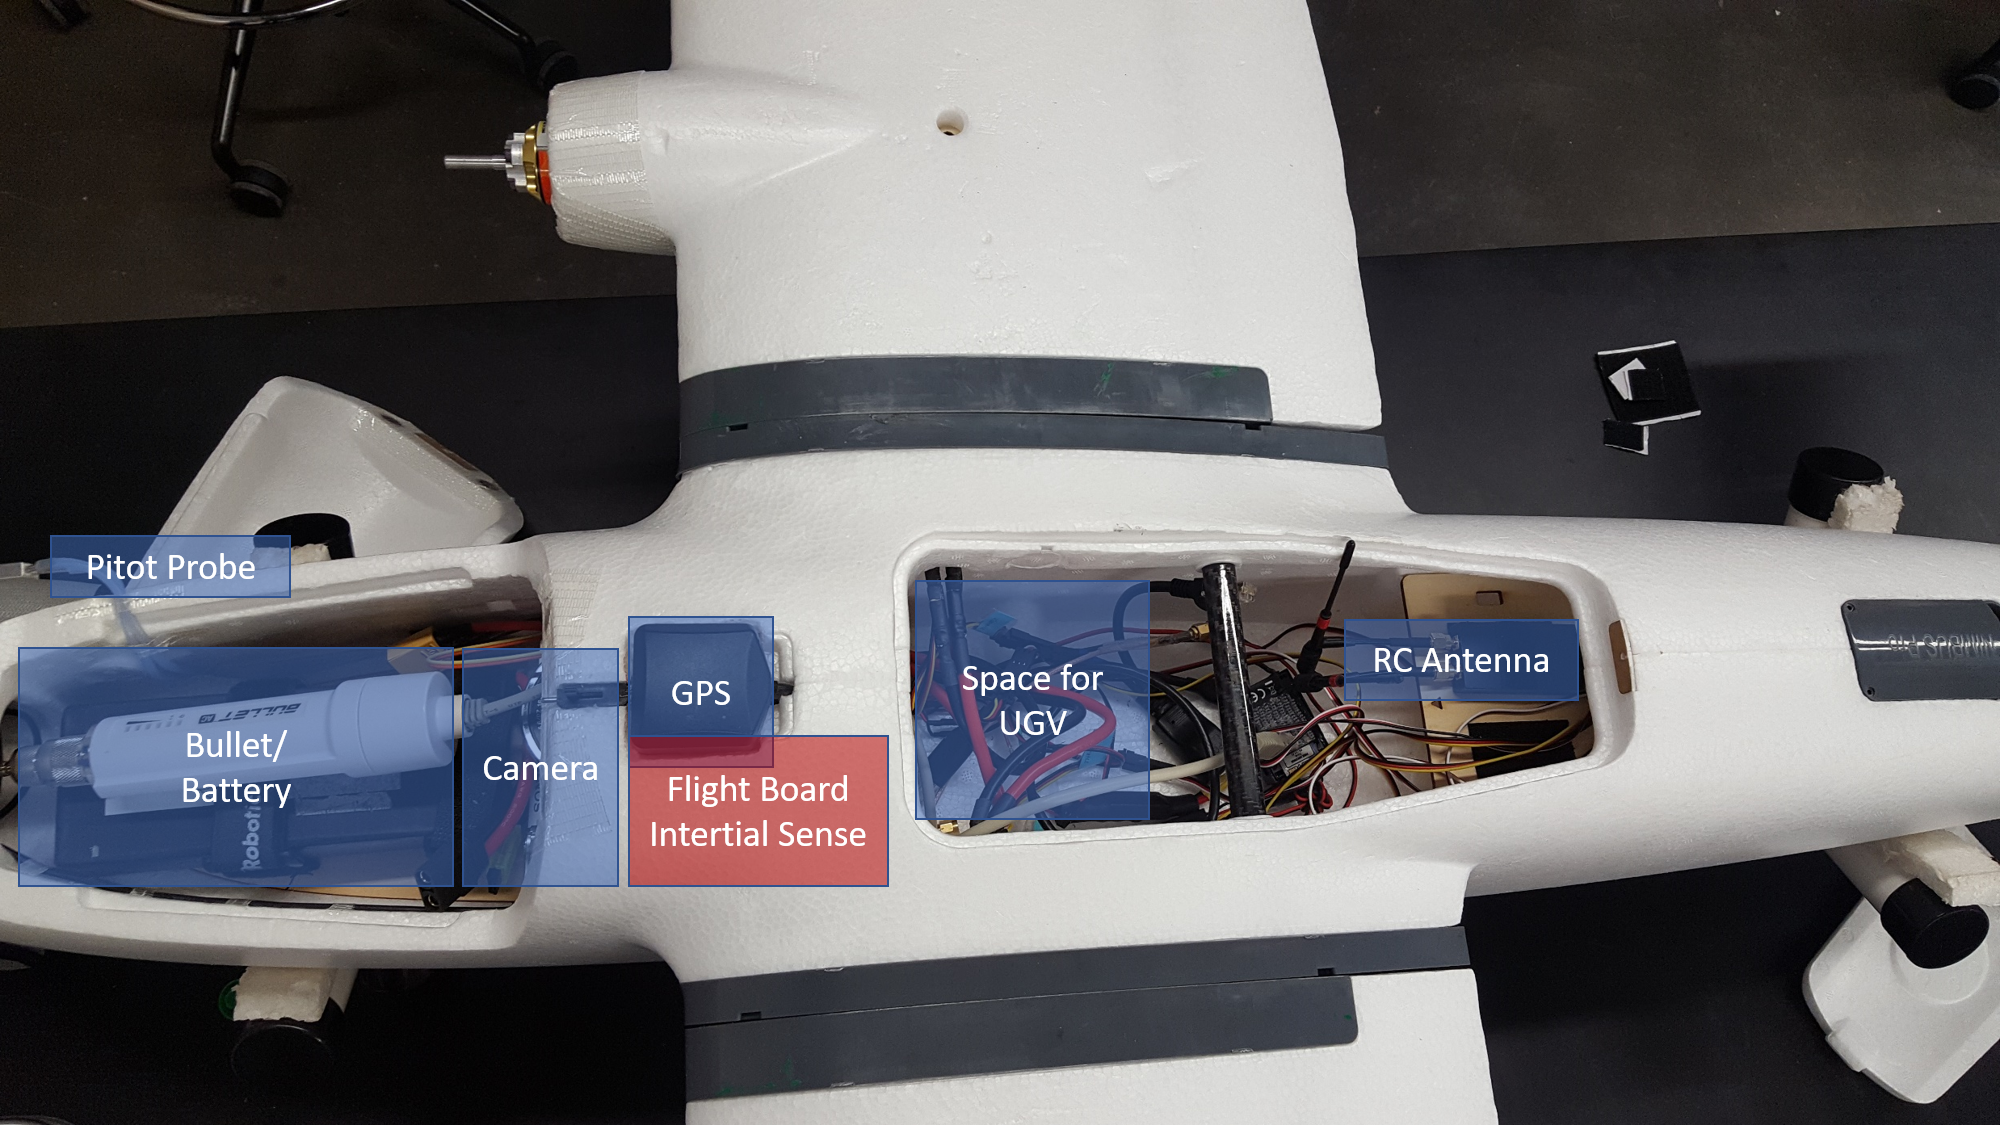
\includegraphics[scale=0.4]{figs/ComponentPlacement.png}
	\centering
	\caption{Component placement is relatively easy in the spacious fuselage. Components are labeled for clarity.}
	\label{components}
\end{figure}
\subsection{Visual Target Classification}
This year's vision team is changing our system architecture for classifying targets which will
allow for better communication and organization. Instead of downloading each image and image state
onto someone's personal computer, the computer oboard the plane will send image and vehicle state
data to a server on the ground. This server will have a compiled database of all images captured
and will attach classification data onto each image as it is manually processed. Our
autonomous detection script will also be querying the server image database and classifying
images. One team member will be monitoring the autonomous output ready to kill the
program if it is sending too many false positives (which cause the team to incur a
penalty).
\subsection{Payload Delivery}
To achieve excellent performance on the key success measure of airdrop accuracy for our unmanned ground vehicle (UGV) payload, the results of our preliminary prototying and testing allowed us to converge on an uncontrolled parachute-deployed payload delivery system. The UGV will be loaded within the aircraft. Given the desired drop location, the autopilot will determine the optimal direction and speed from which to drop the payload, using estimated airspeed conditions. A command from the autopilot will open a small hatch on the bottom of the plane and the UGV will fall out. Strings will attach the UGV to a lightweight fabric parachute with a hole in its center. The fabric parachute will be loaded onto the aircraft in a tube that will allow the UGV to pull it out of the aircraft as it falls. After exiting the aircraft, the parachute will be opened by drag. The drag caused by the fabric will slow down the system enough to allow the UGV to survive impact without damage.
\section{Summary of Expected Performance}
\subsection{Airframe}
The new airframe boasts a design speed of 13~m/s, as modeled in XFLR5. This is a significant 35\% decrease from last year's plane. Flying slower should increase handling for hitting waypoints and executing the payload drop with greater precision. It should also improve image quality. (See the Key Success Measures.) The new airframe also has a fuselage capacity of 8,000~cc: a 7\% increase over last year's plane. This is essential with the addition of a UGV as the required payload in this year's competition, especially since last year's plane didn't have room for even a water bottle inside the fuselage. As a final feature, the new airframe features easily removable wings and tail for easy and quick replacement in the case of a severe crash. This should help satisfy the fast and cheap assembly/rebuild prescribed on the Airframe Requirements Matrix.
\subsection{Visual Target Classification}
The new server system architecture is expected to perform much better for target classification that preveious year's methods. We are
confident in our ability to send images from the camera to our onboard computer and down to our groundstation.

The autonomous classification system is the largest undertaking of this year's vision subteam. Each of the 6 characteristics we are
required to identify could potentially be done using a different method. We expect to be able to reliable classify fifty percent of
targets autonomously.
\subsection{Payload Delivery}
As part of the design process, we have considered multiple points of failure and used those points to inform our design. This, along with the testing documented in the \textit{Unmanned Ground Vehicle Drop Mechanism Concept Test Procedures and Results} artifact, give us confidence that we can achieve an airdrop accuracy within 25 feet from the target drop location, as listed in our key success measures in our Project Contract. In our tests, we evaluated several different delivery mechanisms, and tested for their mass, volume, weight, drag, and drop precision in a controlled environment. These results were weighed against competition requirements for weight and volume, as well as our key success measure concerning drop precision. Our testing convinces us that our chosen payload delivery system, together with refinement and testing of the autopilot drop calculation algorithm, will adhere to the requirements of the competition and allow us to capture our key success measure criteria for excellent performance.
\section{Status and Future Plans}
\subsection{Airframe}
The airframe is currently ready for RC flight testing. Because of a lack of understanding of the complexities of the new airframe, we are behind schedule. Fortunately, it should still be ready for our mock-competition deadline before the end of the semester. Essential components for RC flight have been installed and balanced for the optimal CG placement (as determined using the XFLR5 model), and we have tentative plans for installing the remaining components. The mechanism for releasing the UGV has not yet been constructed, though concept development is already underway, including a dedicated space in the fuselage for it. CG will need to be rebalanced once the UGV is added. More has not yet been done in part because the UGV has not yet been designed. Further testing remains to be done to determine if wing extensions will be necessary. This will probably consist mostly of imaging tests. If image quality is unsatisfactory, then efforts to reduce the design speed by extending the wings will be worthwhile. Otherwise, our time may be better used elsewhere. Further plans for next semester include building and refining the payload mechanism.
\subsection{Visual Target Classification}
We have already built much of the server system architecture. There is a strong framework in place for saving and accessing pictures
from the server. We have also constructed a draft of the user interface that contacts the server and requests images and sends back
cropped and classified images back to the server. The system for manual target recognition is already mostly complete.

We have been focusing on first achieving the ability for manual target recognition, but we have also been investing some effort into developing
the autonomous target detection and classification system. As was mentioned previously, the system must be capable of detecting a target
within a frame, geolocating it, and classifying its shape, shape color, alphanumeric, and alphanumeric color. Thus far, we have developed a
system capable of detecting targets with around 70\% accuracy. We have also modified a deep learning-based character recognition system
to detect synthetic letters with over 90\% accuracy. In the future, we will be working on testing the character recognizer on
real images of targets. We will also be devoloping the shape classifier and color recognition systems.
\subsection{Payload Delivery}
At the outset, our overarching plans were to decide on a payload delivery method, build a prototype, and get last year's payload delivery system up and running. As of right now, we have converged on a method, built a prototype, and tested the software and hardware from last year's system on the ground, but not in the air. Because we have verified that the payload hardware works from last year, the only thing we were not able to do that we planned to do was test the accuracy of the autopilot drop calculation algorithm. We were planning on refining this algorithm anyway, so we will push this step to next semester without much concern.
Next semester, in addition to testing and refining the drop calculation algorithm, we want to build a final version of our parachute delivery system, as well as the UGV payload itself. The majority of our work next semester concerning payload delivery will be iterating the combined payload delivery system (drop calcualtion algorithm, parachute, and UGV) with repeated simulation and hardware testing to ensure repeatability of expected performance in the face of differing environmental conditions, such as wind speed and direction.
\section{Conclusion}
From our design work outlined above and expounded upon in the artifacts below, we are confident that we will be able to construct and refine a product capable of meeting all of our key success measures and performing well in the AUVSI competition.
% document contents
\end{document}
